\documentclass[a4paper]{jsarticle}
\setlength{\baselineskip}{16pt}
\setlength{\parskip}{6mm}

% Packages
\usepackage[top = 20truemm, bottom = 20truemm, left = 30truemm, right = 30truemm]{geometry}
\usepackage{amsmath} % For mathematical equations
\usepackage{cite} % For citations
\usepackage{hyperref} % For hyperlinks
\usepackage[dvipdfmx]{graphicx}
\usepackage{here} % For figure placement

% Title and author
\title{中級ミクロデータサイエンス期末課題\\Problem Set 2}
\author{横浜国立大学経済学部3年\\学籍番号 2125178\\廣江友哉}

\begin{document}

\maketitle

\section*{(a)記述統計}

\subsection*{a-1, 問題背景などを知る上で役に立つ記述統計を作成し、内容について議論しなさい}
\begin{figure}[h]
  \centering
  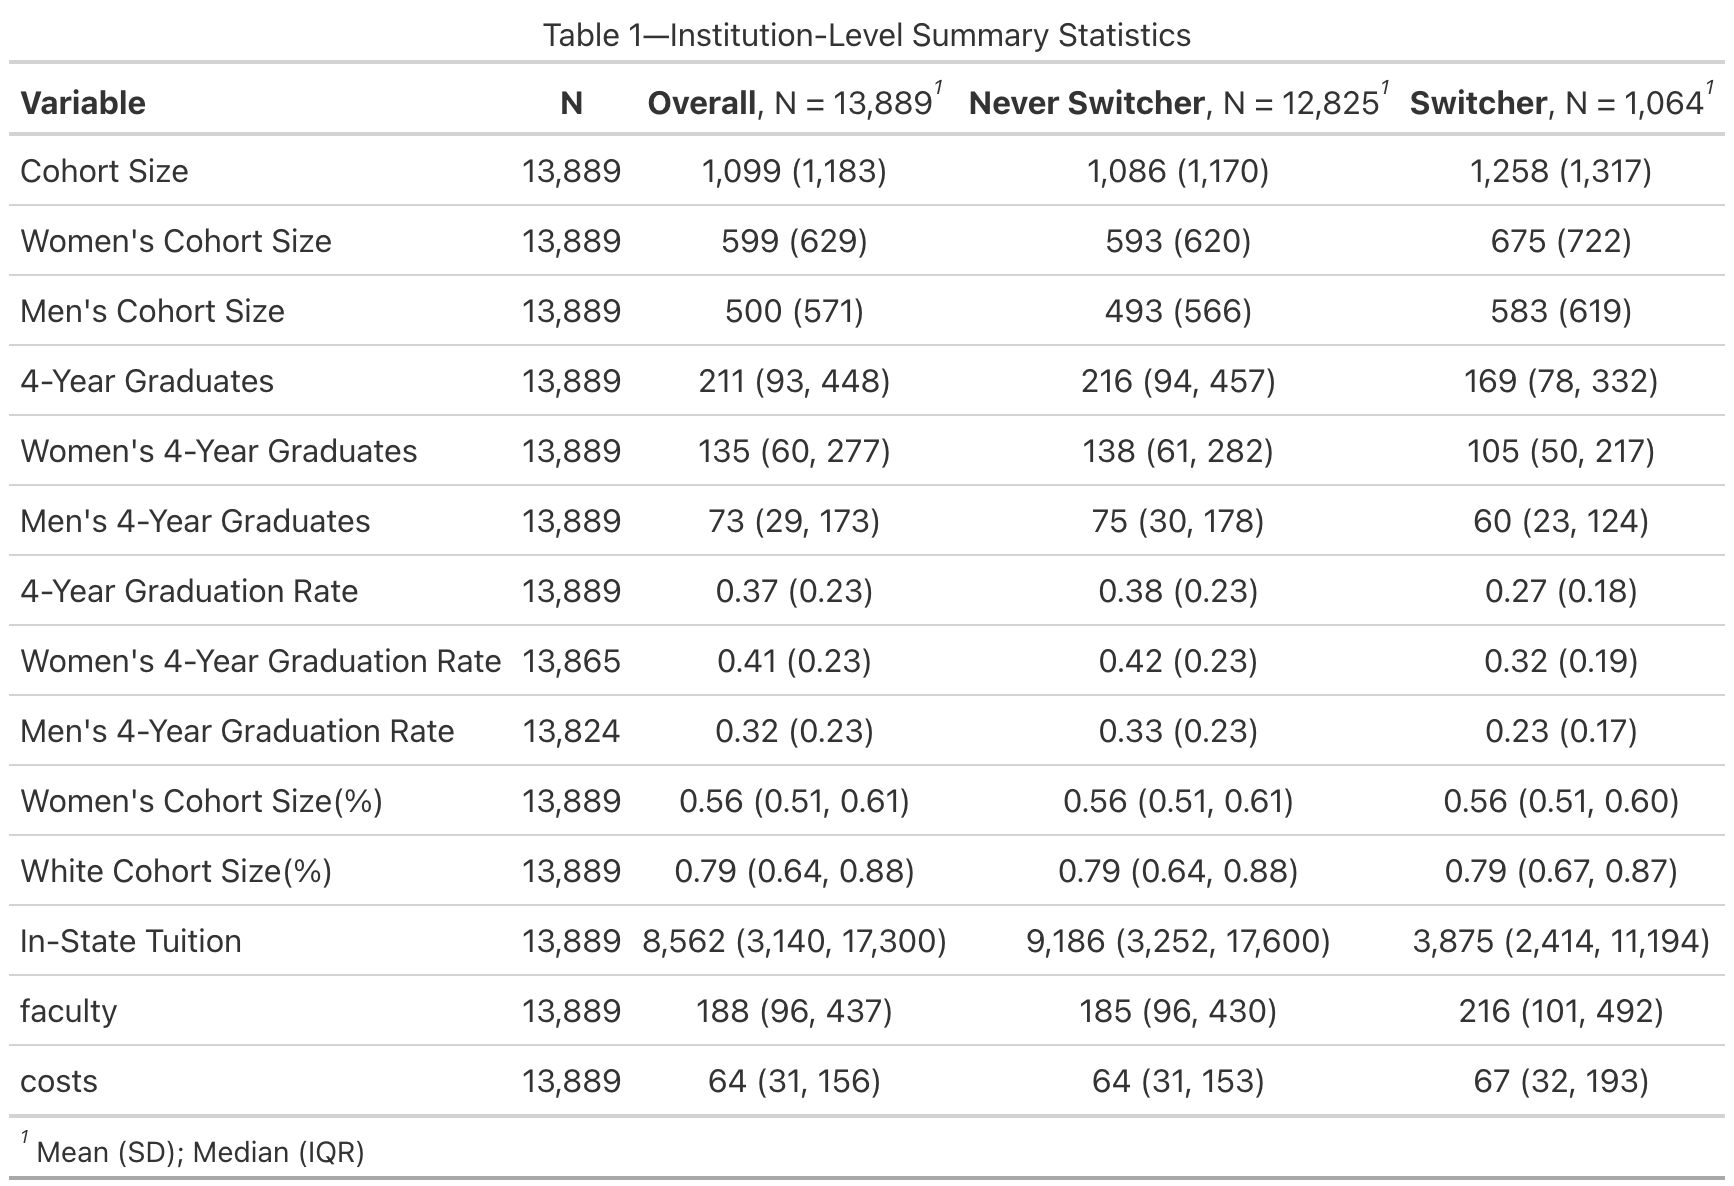
\includegraphics[width = \hsize]{\$HOME/code_box/learn/R/replication-project/src/analyze/output/table/table_1.png}

\end{figure}

クオーター制からセメスター制への移行を1991年から2005年までの間に行った大学は調査対象の大学731校中56校だった。これは元論文の "Switcher"\footnote{Switcher ... クォーター制からセメスター制に変更があった大学} 76校と比較してだいぶ少ない数となっているため、Rで書いたコードの中に誤りが含まれる、もしくは、そもそもの計算方法に誤りがある可能性がある。女性の4年卒業率は男性の四年卒業率と比較して高い傾向にあり、これは "Switcher" "Never Switcher" に関わらず共通している。一方で、卒業率や卒業者数を確認すると、4年卒業率は "Switcher" で 27\% ± 18\%、"Never Switcher" で 38\% ± 23\% となっており、セメスター制に移行することで卒業率が下がる可能性を示唆している。男性についても4年卒業率を確認すると、"Switcher" で 23\% ± 17\%、"Never Switcher" で 33\% ± 23\% となっており、女性は、"Switcher" で 32\% ± 19\%、"Never Switcher" で 42\% ± 23\% となっている。従って性別に関わらず、セメスター制に移行することで卒業率が下がる可能性がある。

\subsection*{a-2, 4年卒業率の平均推移を計算し、図で示しなさい}

各年ごとにすべての大学の4年卒業率の平均を計算し、図で示すと以下のようになる。

\begin{figure}[H]
  \centering
  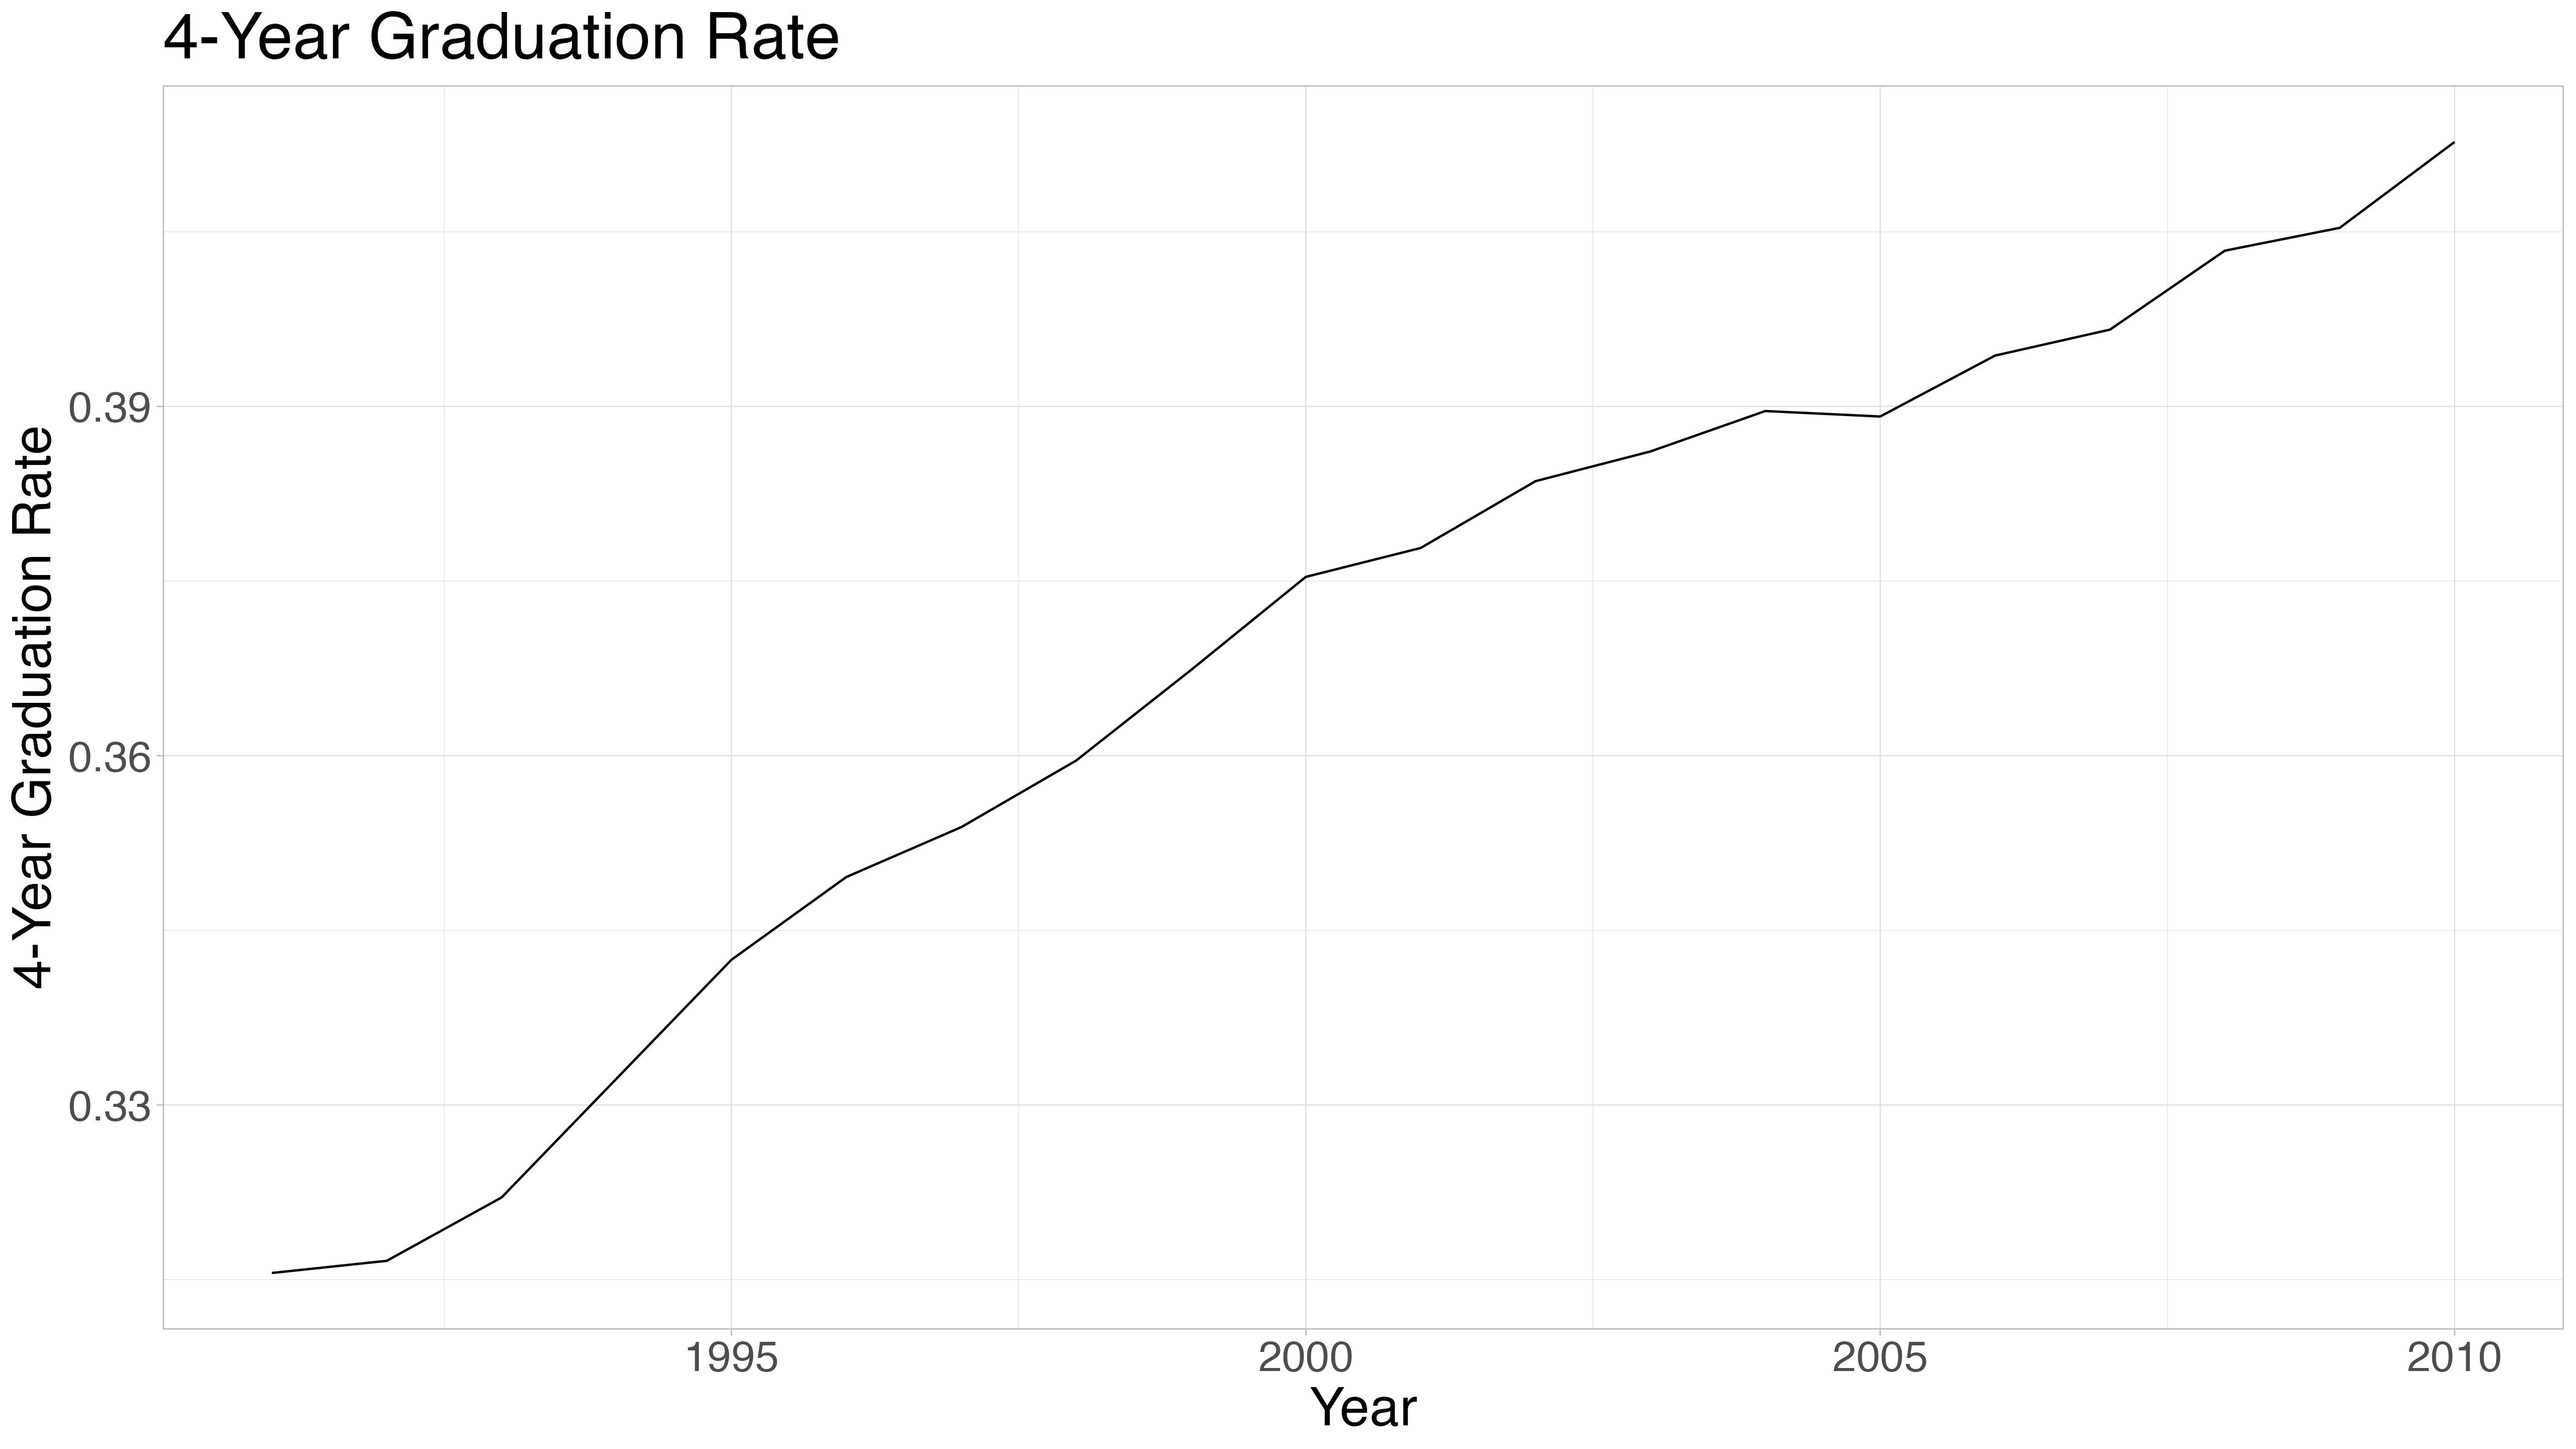
\includegraphics[width = \hsize]{\$HOME/code_box/learn/R/replication-project/src/analyze/output/figure/gradrate_trend.png}

\end{figure}

\subsection*{a-3, semester導入率を計算し、図で示しなさい}

\begin{figure}[H]
  \centering
  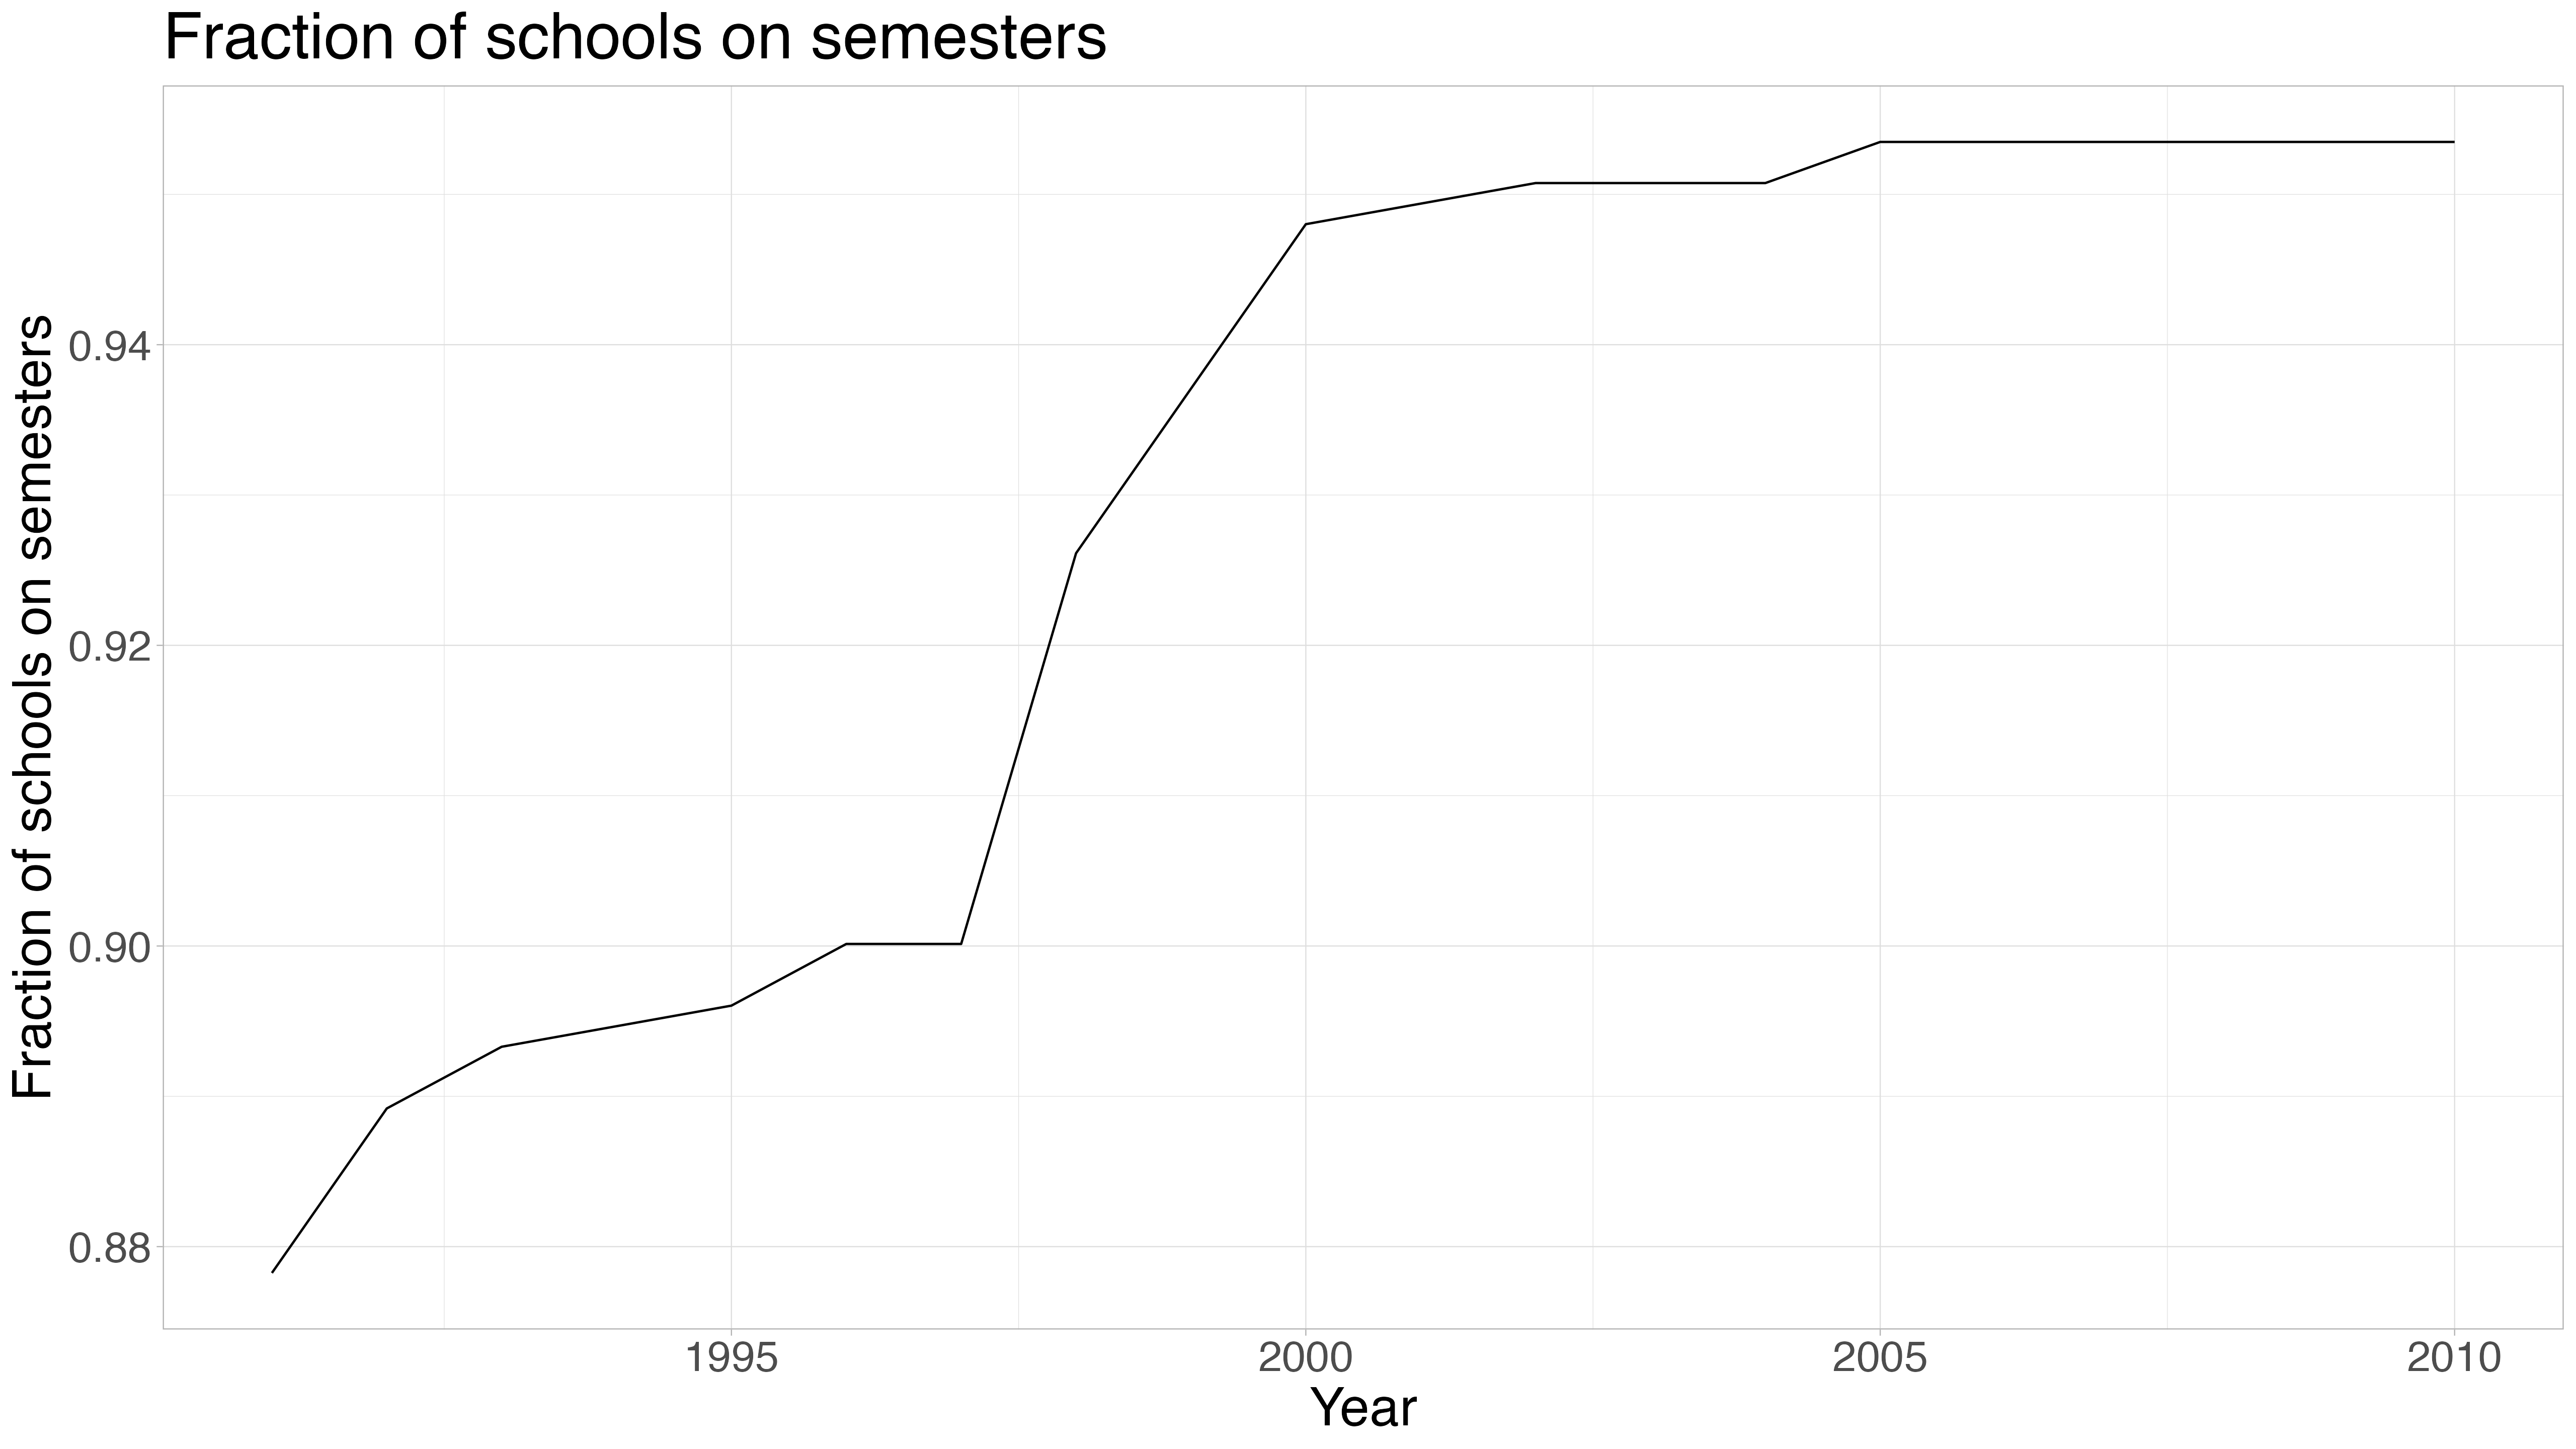
\includegraphics[width = \hsize]{\$HOME/code_box/learn/R/replication-project/src/analyze/output/figure/semester_trend.png}

\end{figure}

\subsection*{a-4, 変数に処理を加えた上で、以下の散布図を作成しなさい。また、重要だと考える結果について議論しなさい}



% Bibliography
\begin{thebibliography}{9}
  \bibitem{textbook}
  中村剛治郎(2020)『基本ケースで学ぶ地域経済学』有斐閣ブックス

  \bibitem{url_module}
  「モジュール化」『神戸大学MBA/ビジネスキーワード』2003年10月15日(\url{https://mba.kobe-u.ac.jp/business_keyword/8000/} 最終アクセス 2024年2月2日)

  \bibitem{us_union_membership_rate}
  Bureau of Labor Statistics, (2024), "Union Member - 2023"

  \bibitem{jp_union_membership_rate}
  厚生労働省(2023)「令和5年労働組合基礎調査の概況」

  \bibitem{us_high_tech_union_membership_rate}
  日本貿易振興機構(ジェトロ)海外調査部 北米課(2014)「北米における労働組合と労働権法制定の動き」:13-17。

  \bibitem{us_start_ups}
  国立研究開発法人科学技術振興機構 研究開発戦略センター(2017)「海外の研究開発型スタートアップ支援」:9-14。

  \bibitem{nda_article}
  「シリコンバレーで日本人が起業するには――“TIME24 VENTURE FESTA99”から」『ASCII.jp』1999年10月6日(\url{https://ascii.jp/elem/000/000/305/305517/} 最終アクセス2024年2月2日)
\end{thebibliography}

\end{document}
